\providecommand{\main}{../..}
\documentclass[\main/thesis.tex]{subfiles}

\begin{document}

\section{Grid Size Comparisons}
In Figure \ref{fig:GridSizeComparisonTimeSteps} we show a sample time-step for each grid size we compare. In (a) the grid size is 64x64, in (b) the grid size is 128x128, in (c) the grid size is 256x256, and in (d) the grid size is 512x512. When comparing the grid sizes all the other parameters were the same, both carcinogens were activated and carcinogen spatial distribution 2 was used. We see that as the domain size increases, the tumour masses within it also increase.
\begin{figure}[H]
    \centering
    \begin{subfigure}[t]{.47\textwidth}
        \centering
        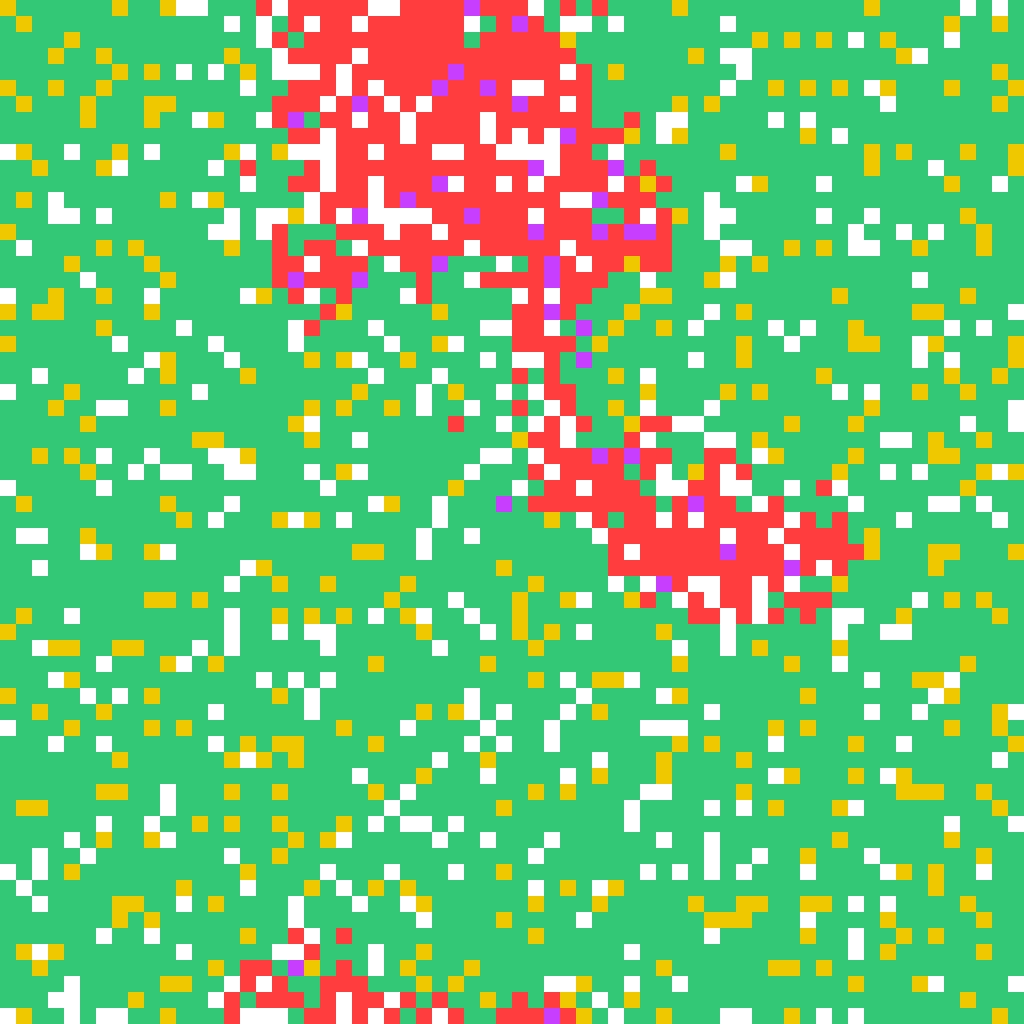
\includegraphics[width=\textwidth]{images/3_GridSizeComparison/Fig1/1_64x64.jpeg}
        \caption{64x64}
        \label{fig:64x64TimeStep}
    \end{subfigure}
    \begin{subfigure}[t]{.47\textwidth}
        \centering
        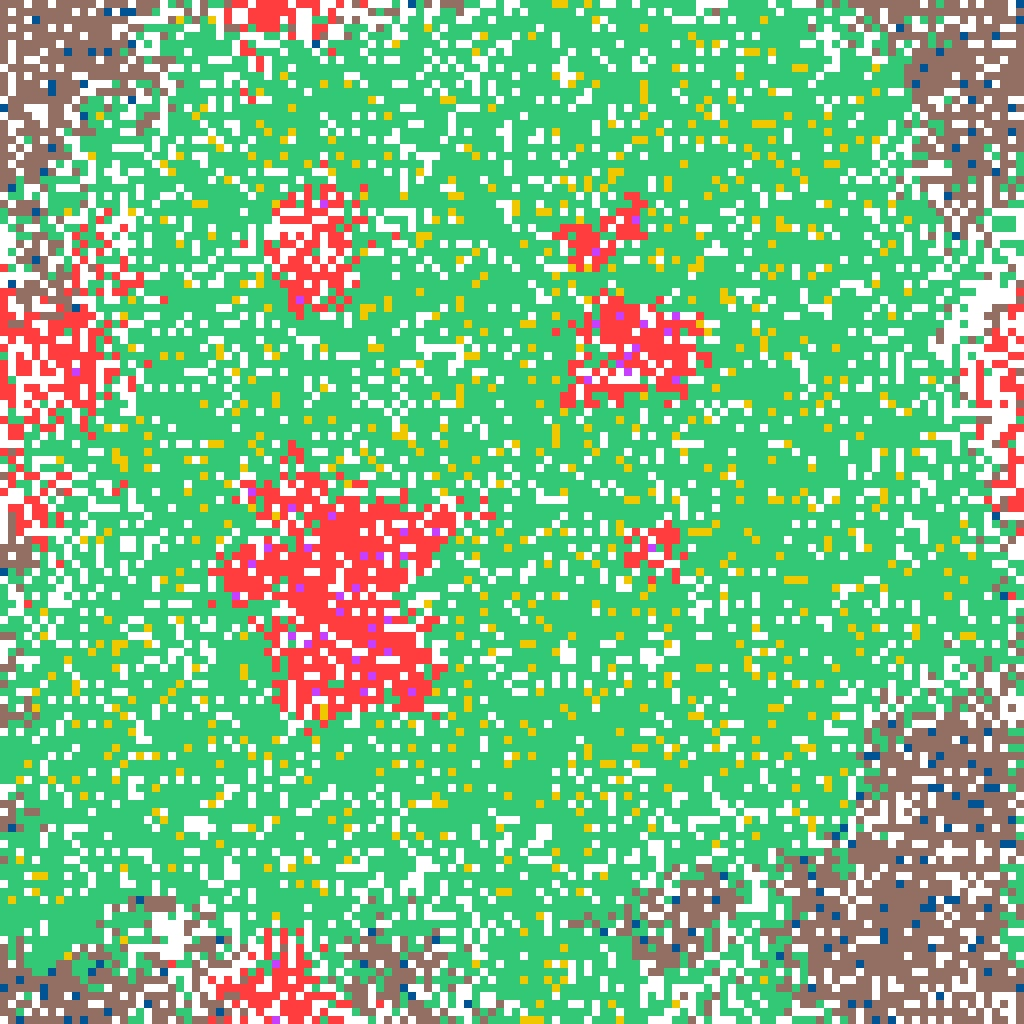
\includegraphics[width=\textwidth]{images/3_GridSizeComparison/Fig1/2_128x128.jpeg}
        \caption{128x128}
        \label{fig:128x128TimeStep}
    \end{subfigure}
    \begin{subfigure}[t]{.47\textwidth}
        \centering
        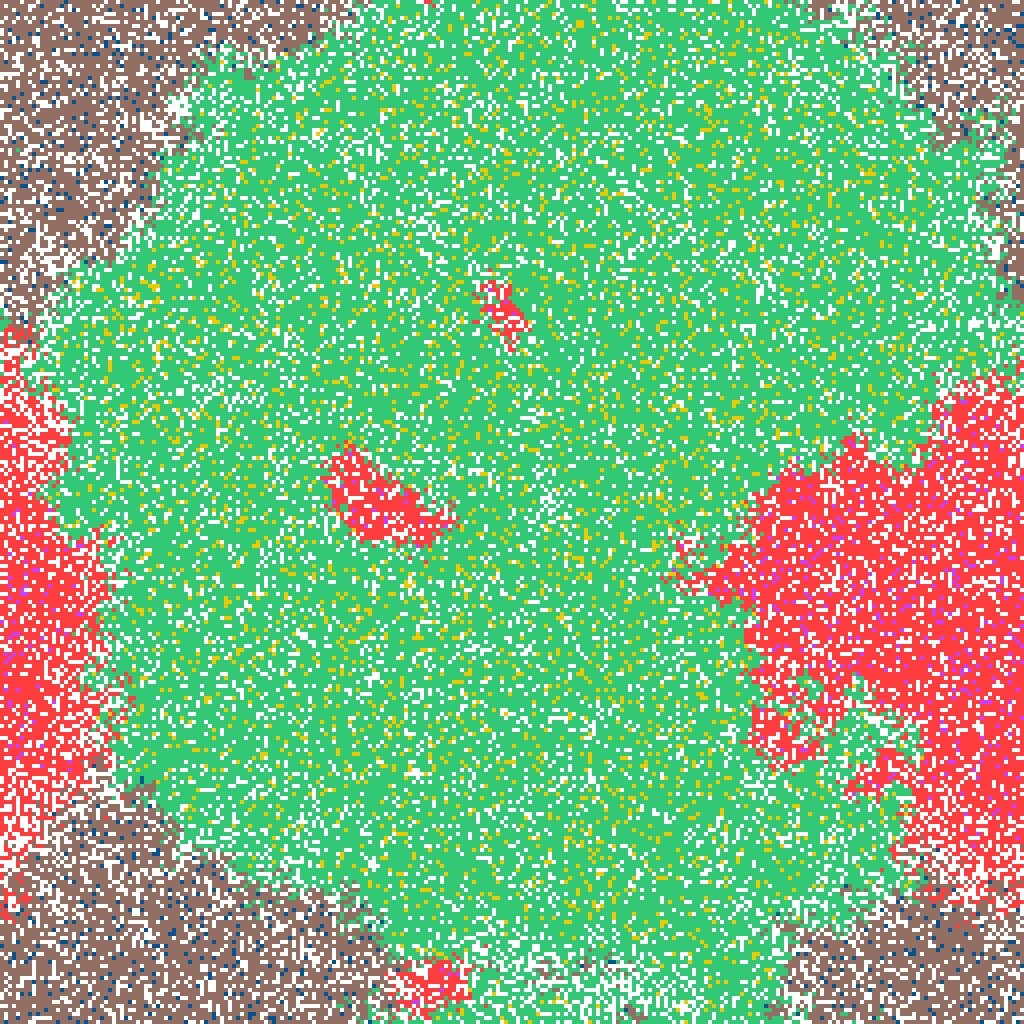
\includegraphics[width=\textwidth]{images/3_GridSizeComparison/Fig1/3_256x256.jpeg}
        \caption{256x256}
        \label{fig:256x256TimeStep}
    \end{subfigure}
    \begin{subfigure}[t]{.47\textwidth}
        \centering
        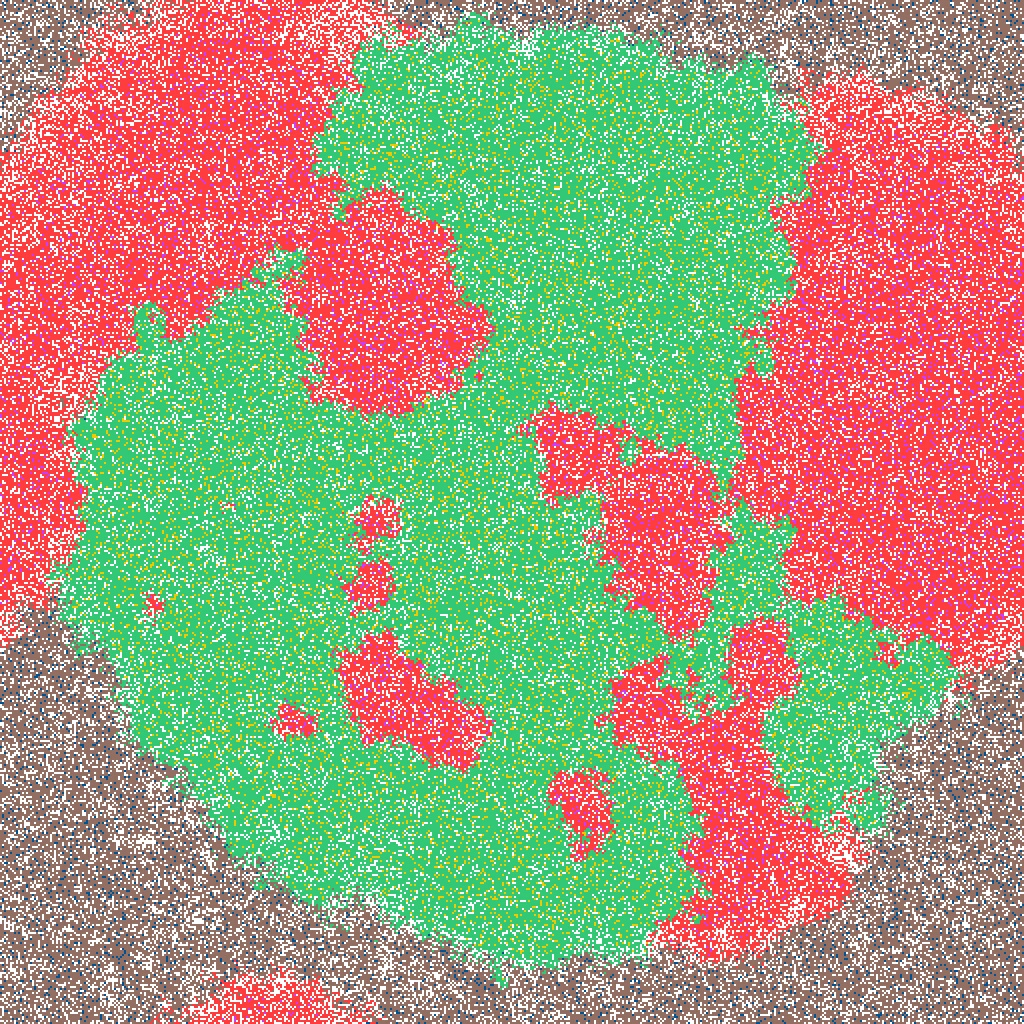
\includegraphics[width=\textwidth]{images/3_GridSizeComparison/Fig1/4_512x512.jpeg}
        \caption{512x512}
        \label{fig:512x512TimeStep}
    \end{subfigure}
    \caption{This figure shows a time-step from each of the grid sizes that were considered for comparison. In (a) the grid size is 64x64, in (b) the grid size is 128x128, in (c) the grid size is 256x256, and in (d) the grid size is 512x512. Parameters: both carcinogens were activated and carcinogen spatial distribution 2 was used.}
    \label{fig:GridSizeComparisonTimeSteps}
\end{figure}
The various grid sizes show slight differences in four ways, all predominantly due to the increase in the number of cells. Most of the events in the CA are probabilistic, as a result, almost automatically, as we increase the size of the grid, the chance of a probabilistic event increases as well. Therefore, the overall dynamics are the same for each grid size, but the timing of various main events differ slightly as will be illustrated with the following tables. 

In Table \ref{table:FirstMutatedCellGridSizeComparison} we show the time-step at which the first mutated cell forms and the cell class of that cell. The time-step indicates no pattern to explain the differences in the values as a consequence of the random effects. We note that the first mutated cell is always an MNTC, due to the fact that a higher ratio of NTC than NSC exists in the domain.
\begin{table}[H]
\centering
\resizebox{\textwidth}{!}{%
\begin{tabular}{|c|c|c|}
	\hline
	Grid size & Time-step first mutated cell forms & Cell class of first mutated cell \\
	\hline
	64x64 & 817 &  MNTC \\
	128x128 & 748 & MNTC \\
	256x256 & 744 & MNTC \\
	512x512 & 735 & MNTC \\
	\hline
\end{tabular}}
\caption{In this table we compare the time-step the first mutated cell forms and the cell class that cell belongs to between the different grid sizes.}
\label{table:FirstMutatedCellGridSizeComparison} 
\end{table}

In Table \ref{table:FirstCSCGridSizeComparison}, we compare the time-step the first CSC forms and the amount of time since the first mutated cell formed for each grid size. The table shows that the variation between the smallest grid size as compared to the remaining three is substantially larger. Due to the fact that the probability of a CSC forming is minuscule, attempting such an action within such a small grid size reduces the chances of these formations drastically in comparison to the larger grid sizes. Similarly, it would be expected that the opposite would be true for the largest grid size in which we observe the shortest time-step to the formation of the first CSC. With regards to the other two grid sizes we observe these to be insignificantly different demonstrating the probabilistic effects influencing the differences. We note that the time-steps since the first mutated cell was formed to the first CSC forms follow the same pattern in that the smallest grid has the largest value and the largest grid has the smallest value. This is expected due to the fact that all four grids formed the first mutated cells at very close time-steps. Overall, grid size in the two outer cases, the smallest and largest, does impact the time it takes for the first CSC to form. 
\begin{table}[H]
\centering
\resizebox{\textwidth}{!}{%
\begin{tabular}{|c|c|c|}
	\hline
	Grid size & Time-step first CSC forms & \# of time-steps since first mutated cell \\
	\hline
	64x64 & 2872 &  2055 \\
	128x128 & 1402 & 654 \\
	256x256 & 1650 & 906 \\
	512x512 & 1082 & 347 \\
	\hline
\end{tabular}}
\caption{In this table we compare the time-step the first CSC forms and the number of time-steps since the first mutated cell formed between the various grid sizes.}
\label{table:FirstCSCGridSizeComparison} 
\end{table}

Table \ref{table:FirstTCGridSizeComparison} compares the time-step the first TC forms and the amount of time since the first CSC formed for each grid size. Note that we observe basically no time lapse between the formation of the first CSC and the first TC, therefore we observe the same differences with the formation of the first TC as we did in the prior observations of the formation of the first CSC. The 128x128 grid formed the first CSC and the first TC simultaneously, this is possible due to a cell’s ability to change cell classes and perform a phenotypic action in the same time-step.
\begin{table}[H]
\centering
\resizebox{\textwidth}{!}{%
\begin{tabular}{|c|c|c|}
	\hline
	Grid size & Time-step first TC forms & \# of time-steps since first CSC \\
	\hline
	64x64 & 2875 & 3 \\
	128x128 & 1402 & 0 \\
	256x256 & 1653 & 3 \\
	512x512 & 1084 & 2 \\
	\hline
\end{tabular}}
\caption{In this table we compare the time-step the first TC forms and the elapsed amount of time it takes a CSC to form the first TC between the various grid sizes.}
\label{table:FirstTCGridSizeComparison} 
\end{table}

In Table \ref{table:PercentFilledGridSizeComparison} we compare the total number of time-steps to the final endpoint, number of time-steps since the first TC formed, and the percentage of the domain occupied by the tumour mass(es) at the endpoint for each of the grid sizes. Recall that the model is set with a loop in which the cells are acting and being acted upon either until a period of 10 years (8776 time-steps) is reached or the grid is composed of only CSC, TC, and empty cells. Note that the two grid sizes that were stopped due to the 10 years rule were the 64x64 and the 512x512. The smaller of these only reached a very small percentage of occupied tumour mass whereas the larger grid size reached similar percentages as the other two. Since the smallest grid size has insufficient cell numbers, the law of large numbers does not come into play and thus the chance of various events is too low, as a result it does not form a tumour aggressive enough to fill the majority of the domain within 10 years. With regards to the 512x512 grid size the 10 year rule stopped the tumour from further developing simply due to the vast number of cells within the domain increasing the number of time-steps. When comparing the 128x128 to the 256x256 in which the simulation ended before the 10 years, then the smaller grid size took less time to reach a similar percentage occupied of tumour mass due to a combination of less space to overcome and less competition between cell lineages. A smaller total number of time-steps is correlated with a cancer field and tumour mass(es) being more aggressive as observed with the 128x128 grid showing the lowest number of time-steps from the first TC being formed to the endpoint.
\begin{table}[H]
\centering
\resizebox{\textwidth}{!}{%
\begin{tabular}{|c|c|c|c|}
	\hline
	Grid size & Total \# time-steps & \# time-steps since first TC & \% occupied by tumour mass(es)\\
	\hline
	64x64 & 8766 & 5891 & 28.44\% \\
	128x128 & 5398 & 3996 & 84.45\% \\
	256x256 & 7995 & 6342 & 86.05\% \\
	512x512 & 8766 & 7682 & 86.51\% \\
	\hline
\end{tabular}}
\caption{This table compares the total number of time-steps, number of time-steps since the first TC formed, and the percentage the tumour mass(es) make up of the domain at the end of the simulation between all the grid sizes.}
\label{table:PercentFilledGridSizeComparison} 
\end{table}

In Table \ref{table:numLineagesGridSizeComparison} we show the number of tumour cell lineages at the end of the simulation for each grid size. Comparing the number of distinct tumour cell lineages between the grid sizes in Table \ref{table:numLineagesGridSizeComparison}, we see an increase relative to grid size. Since all the other lineages either died out or were overthrown via competition, the first two grid sizes end with a domain that has only one tumour cell lineage. Overall, for all the grid sizes, the number of tumour cell lineages decreases over time as the system reaches an equilibrium, where the most fit lineages survive. 
\begin{table}[H]
\centering
\begin{tabular}{|c|c|}
	\hline
	Grid size & \# of tumour cell lineages\\
	\hline
	64x64 & 1 \\
	128x128 & 1 \\
	256x256 & 6 \\
	512x512 & 24 \\
	\hline
\end{tabular}
\caption{In this table we compare the number of tumour cell lineages at the end of the simulation between each of the grid sizes.}
\label{table:numLineagesGridSizeComparison} 
\end{table}

Due to how the parameters for the gene expression neural network were set, such as TP53 influencing all the other genes, comparing all the grid sizes result in all the genes becoming positively mutated.

\end{document}